\chapter{\#45: European transportation networks I}

\resp{Robin Chan}

\section{Introduction}
 
For this task the rail network of Europe and a selection of its countries will be generated using GIS-data provided by the professor. The data originates from EuroGeographics. It contains GIS data for administrative boundaries, hydrography, named locations, settlements and transportation. The latter is of interest for this project. The transportation data includes (not exclusively) ferry lines, airports, roads, level crossings, ... and most interesting for this project, rail lines.

To generate the rail networks, python and mainly the GeoPandas and Pandas libraries were used as the former is well-suited to working with GIS data.

\section{How to extract the relevant data?}

The task is now to find the files containing information about the train stations (nodes) and train lines (edges). Among the wealth of GIS-files these can be identified as \textit{RailrdC} and \textit{RailrdL} respectively.\\

All the relevant information can be found in the shapefiles (.shp). At first it seemed that there was a mismatch between the coordinates of railway stations and railroad boundaries. So it was decided to link nodes to edges based on their vicinity. This, however, would not yield a physical network. Railway lines are not straight lines between stations, but curve around geographic features, population centres, etc. So not all of their boundaries will coincide with railway stations. This can result in railway lines being connected to stations that they are not actually connected to.

The next strategy was to construct the nodes dataframe using all allowed connections to edges. According to the data user manual, RailrdL can connect to RailrdC, ExitC, FerryC and LevelcC (level crossing). Then this dataframe can be filtered by looking at which coordinates correspond to edge coordinates. However, some edges have bounderies on nodes that have no label, they just indicate a location where the rail line changes direction. This causes issues linking edges to to and from coordinates of nodes as not all nodes that rail lines connect are included.

The solution is to construct the nodes dataframe based on the coordinates of the rail line boundaries. Then this can be referenced to the existing (allowed) node coordinates. This allows for labelling of the known nodes, those that do not appear in the searched nodes are labelled as 'unknown'.

\section{Results}

To get an idea if the generated network is correct, we can use matplotlib and geopandas to directly plot the network edges from the shapefile. This can then be compared to the network generated by the procedure described in the previous section.

\begin{figure}[H]
    \centering
    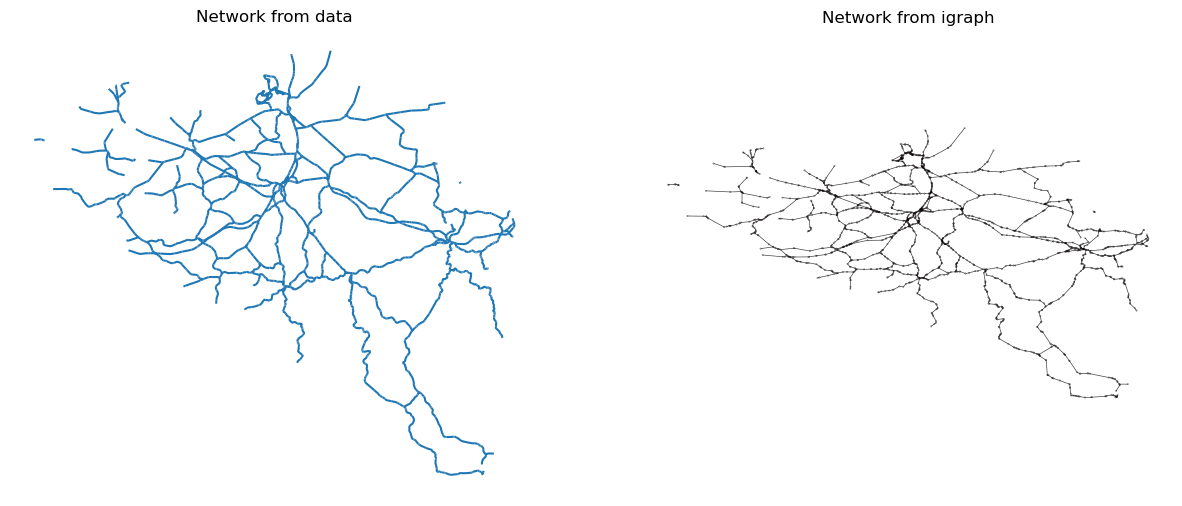
\includegraphics[width=\linewidth]{images/Comparison.png}
    \caption{\textit{Network shown straight from the data (left) and after the filtering procedure, visualised with igraph (right). The strange aspect ratio of the right image is probably due to the way igraph interfaces with matplotlib.}}
    \label{rail_comparison}
\end{figure}

The Belgian network was used as a way of testing the code as I am most familiar with it, being from Belgium myself. I noticed that some lines are not complete (see the northwestern corner). One of these is a major line connecting the coast to the rest of the country. This might be due to the data being taken during a period where works were being performed on the line.

\newpage

\begin{figure}[H]
    \centering
    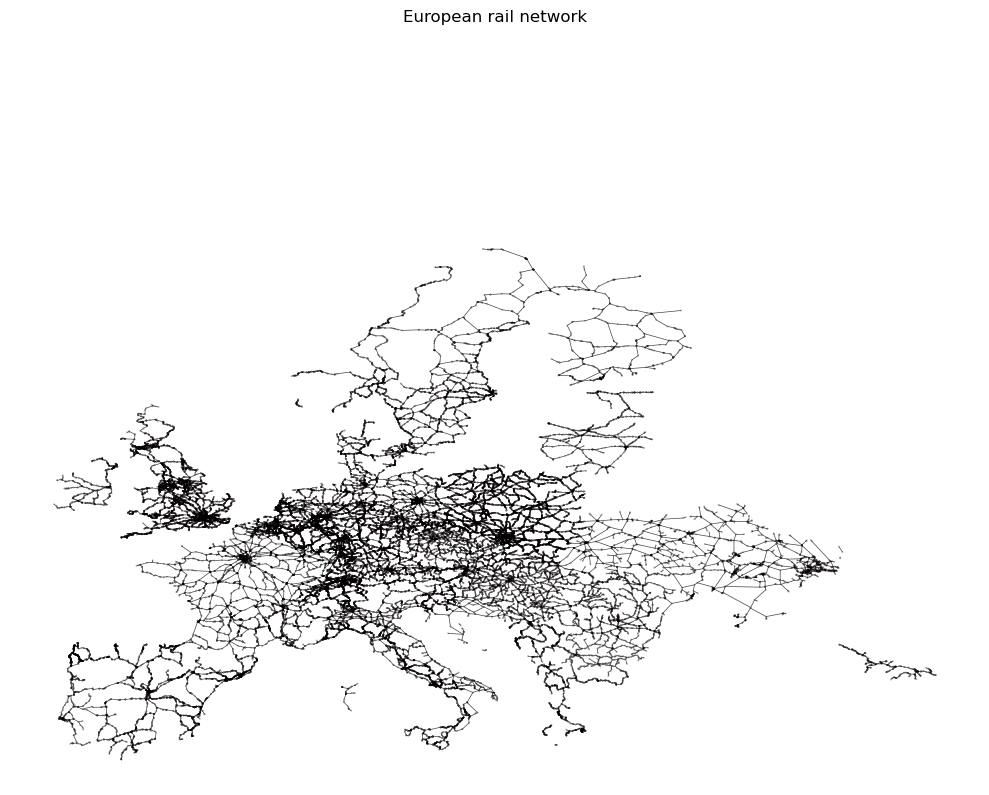
\includegraphics[width=\linewidth]{images/Europe_rail.png}
\end{figure}

\newpage